% Options for packages loaded elsewhere
\PassOptionsToPackage{unicode}{hyperref}
\PassOptionsToPackage{hyphens}{url}
%
\documentclass[
]{article}
\usepackage{amsmath,amssymb}
\usepackage{lmodern}
\usepackage{iftex}
\ifPDFTeX
  \usepackage[T1]{fontenc}
  \usepackage[utf8]{inputenc}
  \usepackage{textcomp} % provide euro and other symbols
\else % if luatex or xetex
  \usepackage{unicode-math}
  \defaultfontfeatures{Scale=MatchLowercase}
  \defaultfontfeatures[\rmfamily]{Ligatures=TeX,Scale=1}
\fi
% Use upquote if available, for straight quotes in verbatim environments
\IfFileExists{upquote.sty}{\usepackage{upquote}}{}
\IfFileExists{microtype.sty}{% use microtype if available
  \usepackage[]{microtype}
  \UseMicrotypeSet[protrusion]{basicmath} % disable protrusion for tt fonts
}{}
\makeatletter
\@ifundefined{KOMAClassName}{% if non-KOMA class
  \IfFileExists{parskip.sty}{%
    \usepackage{parskip}
  }{% else
    \setlength{\parindent}{0pt}
    \setlength{\parskip}{6pt plus 2pt minus 1pt}}
}{% if KOMA class
  \KOMAoptions{parskip=half}}
\makeatother
\usepackage{xcolor}
\IfFileExists{xurl.sty}{\usepackage{xurl}}{} % add URL line breaks if available
\IfFileExists{bookmark.sty}{\usepackage{bookmark}}{\usepackage{hyperref}}
\hypersetup{
  hidelinks,
  pdfcreator={LaTeX via pandoc}}
\urlstyle{same} % disable monospaced font for URLs
\usepackage{graphicx}
\makeatletter
\def\maxwidth{\ifdim\Gin@nat@width>\linewidth\linewidth\else\Gin@nat@width\fi}
\def\maxheight{\ifdim\Gin@nat@height>\textheight\textheight\else\Gin@nat@height\fi}
\makeatother
% Scale images if necessary, so that they will not overflow the page
% margins by default, and it is still possible to overwrite the defaults
% using explicit options in \includegraphics[width, height, ...]{}
\setkeys{Gin}{width=\maxwidth,height=\maxheight,keepaspectratio}
% Set default figure placement to htbp
\makeatletter
\def\fps@figure{htbp}
\makeatother
\setlength{\emergencystretch}{3em} % prevent overfull lines
\providecommand{\tightlist}{%
  \setlength{\itemsep}{0pt}\setlength{\parskip}{0pt}}
\setcounter{secnumdepth}{-\maxdimen} % remove section numbering
\ifLuaTeX
  \usepackage{selnolig}  % disable illegal ligatures
\fi

\author{}
\date{}

\begin{document}

\hypertarget{wind-farms-conclusions}{%
\section{Wind Farms Conclusions}\label{wind-farms-conclusions}}

Teo Zeng

This document attempts to summarize all the observations from the
exploratory data analysis done the forcast and actual wind farm
production in Texas.

\hypertarget{notations}{%
\subsection{Notations}\label{notations}}

\begin{array}{lr}
J & \text { Number of assets } \\
d=1, \ldots, D ; h & \text { Days, Hours } \\
C_i & \text{Capacity for Asset i}\\
\mathbf{g}_{d} = (g_{d,h}) & \text{Actual Production MWh}\\
\mathbf{f}_{d} = (f_{d,h}) & \text{forcasted Production MWh}\\
\tilde{\beta}_{d,h} & \text{prediction bias}\\
i & \text{assets indices}\\
\alpha_{d, h} & \text { actuals fraction } \in[0,1] \\
\gamma_{d, h} & \text { forecast fraction } \in[0,1]\\
\beta_{d,h} & \text{bias fraction} \\
q_{d,h} & \text{95 quantile fraction} \\
\mathbf{q}_{d,h} & \text{quantile}\\
\tau_{d,h} & \text{kendall's tau}\\
r^2 & \text{corelation coefficient}\\
\sigma & \text{normalized standard deviation of bias}\\
\tilde{\sigma} & \text{unnormalized standard deviation of bias}\\
S & \text{the set of all assets}\\
n & \text{number of occurence as outliers}
\end{array}

\begin{itemize}
\item
  Days are indexed by \(d = 1,2,...,365\), and hours are indexed by
  \(h = 1,2,...,24\)
\item
  \(\mathbf{g}_{d,h},\)
  \(\mathbf{f}_{d,h}, \alpha_{d, h}, \beta_{d, h}, q_{d,h}\) are vectors
  of Dimension \(J\) Where
\end{itemize}

\[\alpha_{d,h}\in [0,1] = \frac{\mathbf{g}_{d,h}}{C} \quad \text{and} \quad \gamma_{d,h} \in [0,1] = \frac{\mathbf{f}_{d,h}}{C}\]

\begin{itemize}
\item
  The bias fraction is then
\end{itemize}

\[\beta_{d,h} =  \alpha_{d,h} - \gamma_{d,h}\]

\begin{itemize}
\item
  For a population, of discrete values or for a continuous density, the
  \(k^{th}\) q-quantile is the data value where the cumulative
  distribution function crosses \(k/q\). \(x\) is a \(k^{th}\)
  q-quantile for a variable \(X\) if

  \[\operatorname{Pr}[X<x] \leq k / q \quad \text{and} \quad\operatorname{Pr}[X \leq x] \geq k / q\]
\end{itemize}

\begin{itemize}
\item
  For the entire article, we let \(q =95\), therefore, the quantile for
  an asset at a given time interval is calculated as

  \[\mathbf{q}_{d,h} = q_{d,h} - \bar{\beta}_{d,h}\]
\end{itemize}

\hypertarget{bias}{%
\subsection{Bias}\label{bias}}

\hypertarget{bias-at-hourly-interval}{%
\subsubsection{Bias at hourly interval}\label{bias-at-hourly-interval}}

For a given asset, let

\[\beta_{h} = \frac{1}{365}\sum_{d = 1}^{365} \beta_{d,h}\]

and \(\beta_h\) is the prediction bias for a given hour of the day. For
each \(h \in [1,24]\), we plot out \(\beta_h\) in a violin plot and a
box plot.

\begin{figure}
\centering
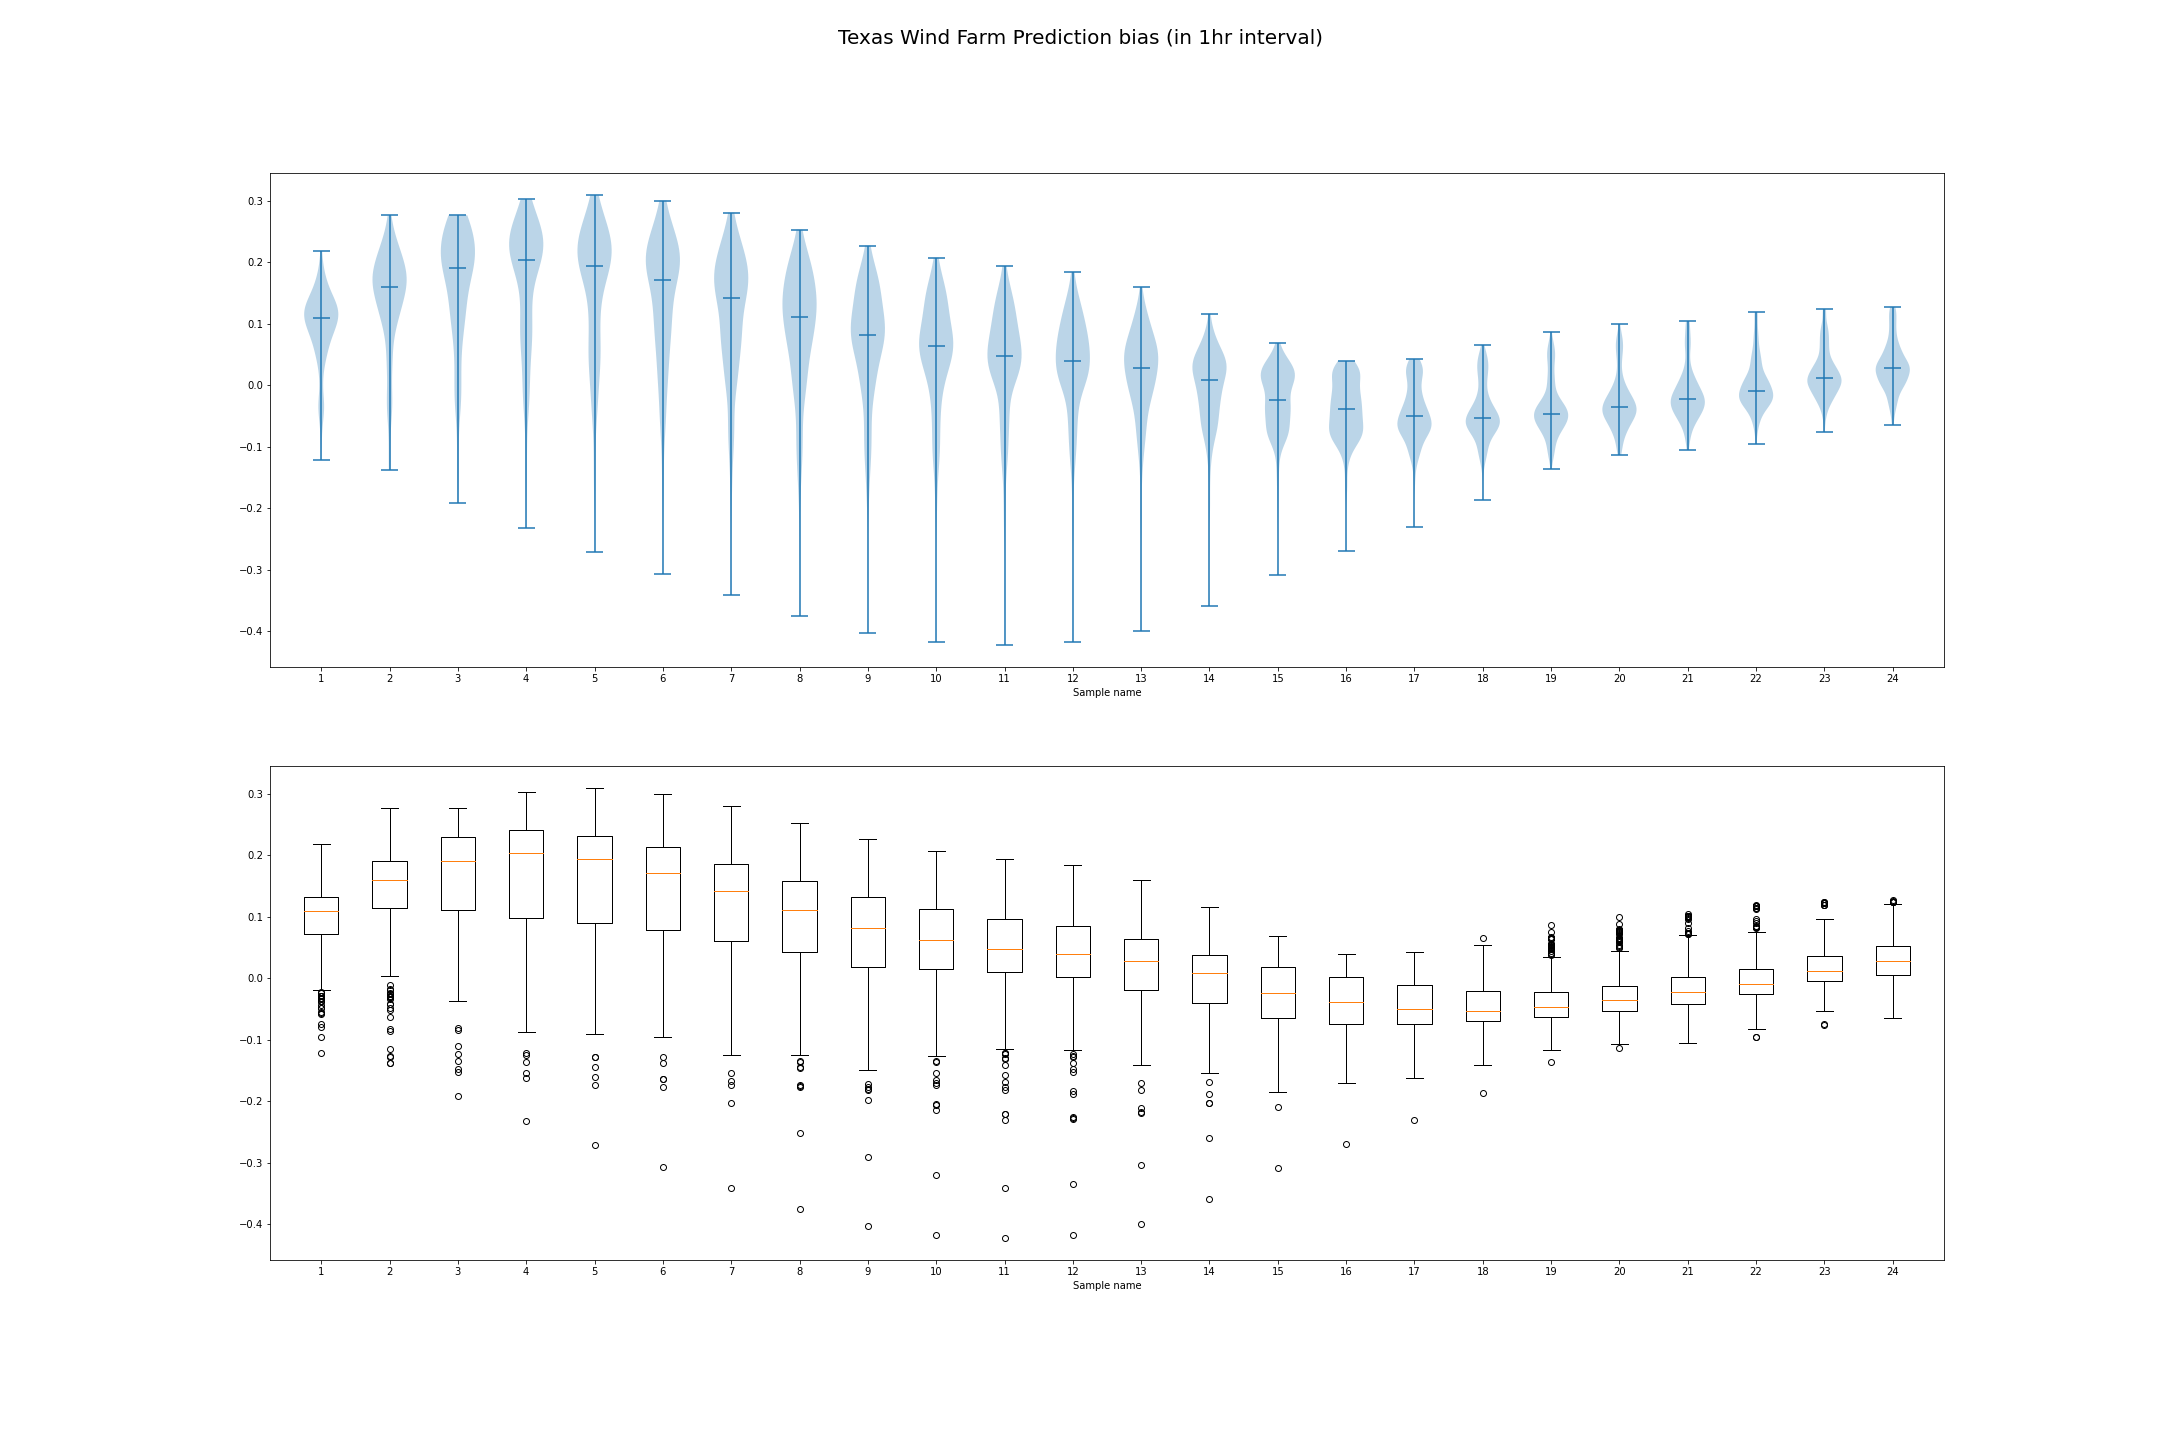
\includegraphics{/Users/teo/Desktop/wind/plots/violin_and_box_bias_1hr.png}
\caption{Violin and Box of Bias at 1 Hour Interval}
\end{figure}

The blue line on the violin plot and the red line on the box plot
represent the median of the data. It was found that, overall in the
morning the prediction bias tend to be positive, with negatively skewed
distribution. In the afternoon and evening the prediction bias tend to
be negative, with less skewed distribuiton. With closer analysis on the
outliers, two outliers at the bottom from hour 3 to hour 19 are due to
\textbf{Canadian Breaks Wind} and \textbf{Desert Sky repower}.

\hypertarget{bias-at-24-hours-interval}{%
\subsubsection{Bias at 24 Hours
interval}\label{bias-at-24-hours-interval}}

We are also interested in the geographic distribution of the prediction
bias.

For a given asset, let

\[\beta = \frac{1}{365\times 24}\sum_{d = 1}^{365} \sum_{h = 1}^{24} \beta_{d,h}\]

and \(\beta\) is also a vector of length \(J\). Plotting \(\beta\) on
the map of Texas,

\begin{figure}
\centering
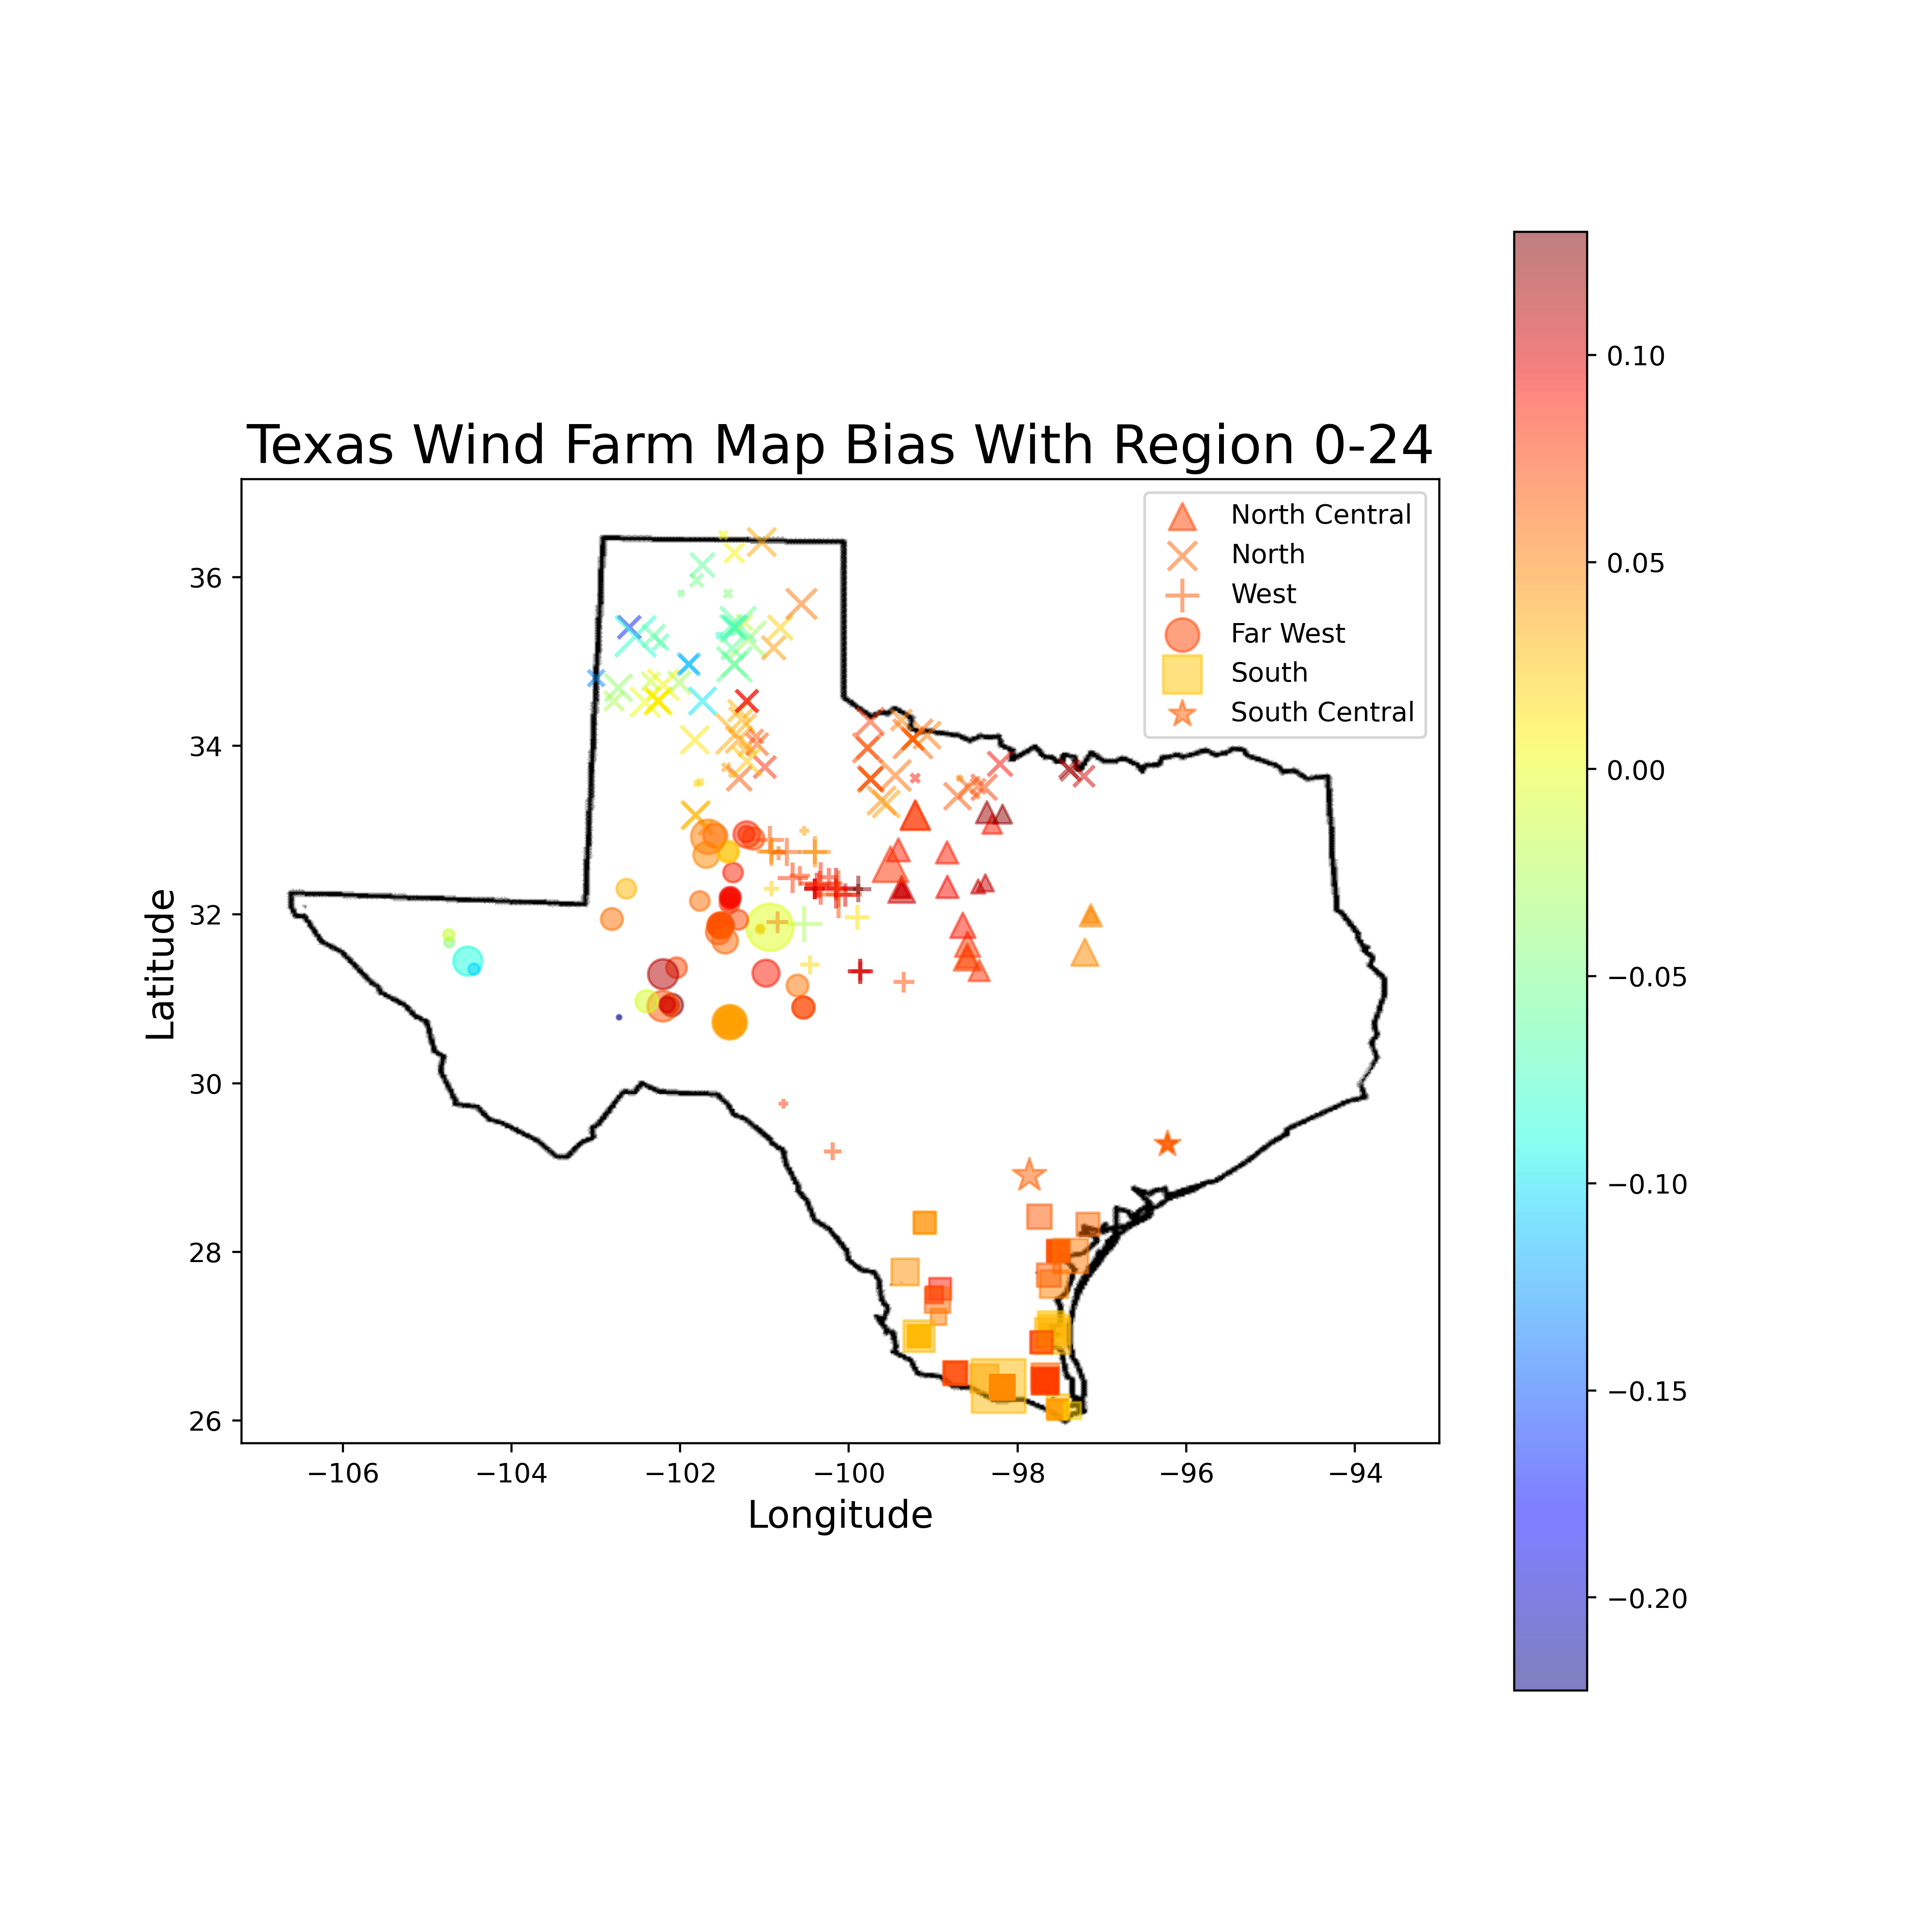
\includegraphics{/Users/teo/Desktop/wind/plots/bias_24hr_with_area.png}
\caption{Bias at 24-hour Interval}
\end{figure}

As observed from the scatter plot, the bias, across all hours and all
year, is relatively higher for Southern and central wind farms and is
lower for Northern and Western windfarms.

\hypertarget{stardard-deviation-of-bias}{%
\subsection{Stardard Deviation of
Bias}\label{stardard-deviation-of-bias}}

\hypertarget{standard-deviation-of-bias-at-hourly-interval}{%
\subsubsection{Standard Deviation of Bias at Hourly
Interval}\label{standard-deviation-of-bias-at-hourly-interval}}

We are also interested in the standard deviation of the Bias. Let

\[\sigma_{h}=\sqrt{\frac{\sum_{d = 1}^{365}\left(\beta_{d,h}-\bar{\beta_h}\right)^{2}}{365}}\]

where \(\bar{\beta_h} = \frac{1}{365}\sum_{d = 1}^{365} \beta_{d,h}\) is
the mean of the bias at a given hour across all year. For each
\(h \in [1,24]\), we plot out \(\sigma_h\) in a violin plot and a box
plot.

\begin{figure}
\centering
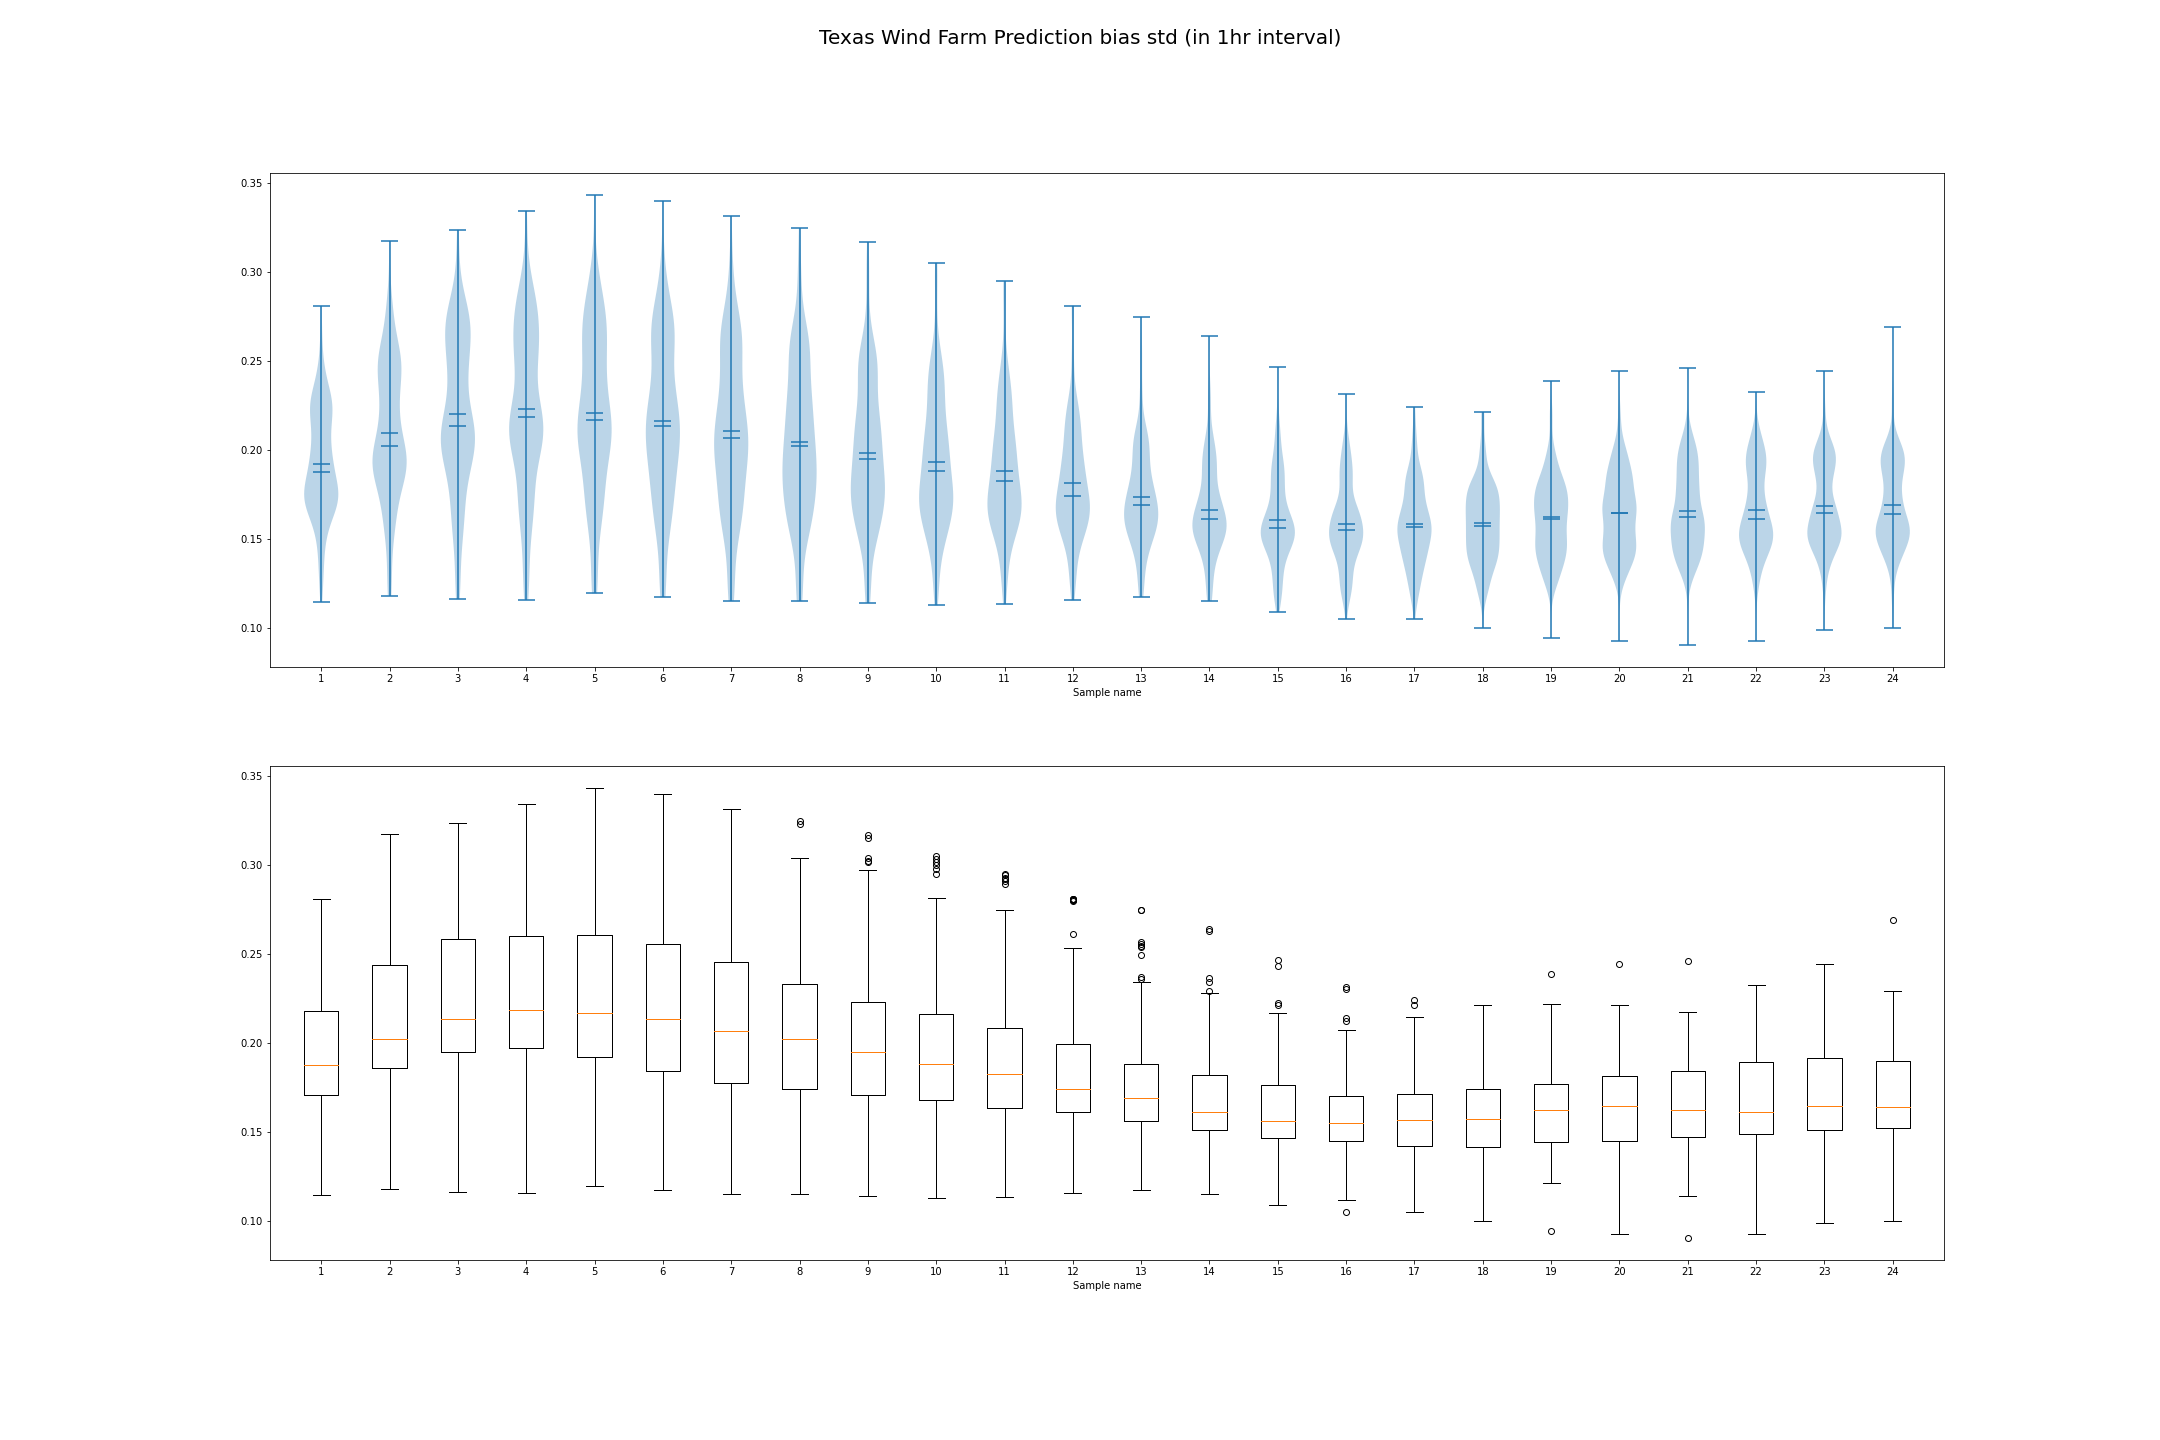
\includegraphics{/Users/teo/Desktop/wind/plots/violin_and_box_std_of_bias_1hr.png}
\caption{Violin and Box of std at 1 Hour Interval}
\end{figure}

It was found that, from the above violin/box plot, the mean and median
of the standard deviation of bias tend to be stable across 24 hours.
There are some outliers during sunlight time and few outliers at night.
It was also found that the standard deviation of bias tend to be larger
in the early morning comparing to the afternoon.

\hypertarget{standard-deviation-of-bias-at-24-hour-interval}{%
\subsubsection{Standard Deviation of Bias at 24 hour
interval}\label{standard-deviation-of-bias-at-24-hour-interval}}

We are also interested in the geographic distribution of the standard
deviation of bias.

For a given asset, let

\[\sigma=\sqrt{\frac{\sum_{h = 1}^{24}\sum_{d = 1}^{365}\left(\beta_{d,h}-\bar{\beta}\right)^{2}}{365}}\]

where
\(\bar{\beta} = \frac{1}{365\times 24}\sum_{h = 1}^{24}\sum_{d = 1}^{365} \beta_{d,h}\)
is the mean of the bias across all year and all hours. \(\sigma\) is
also a vector of length \(J\).

\begin{figure}
\centering
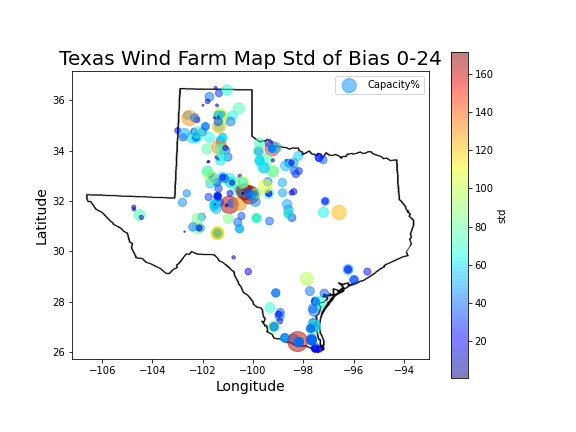
\includegraphics{/Users/teo/Desktop/wind/plots/std_of_bias_24hr.png}
\caption{Standard Deviation of Bias at 24 hour
interval}
\end{figure}

From this scatter plot, it was found that the stardard devaition of bias
is relatively lower for the Southern assets.

\hypertarget{quantile-of-bias}{%
\subsection{Quantile of Bias}\label{quantile-of-bias}}

\hypertarget{quantile-of-bias-at-hourly-interval}{%
\subsubsection{Quantile of Bias at Hourly
Interval}\label{quantile-of-bias-at-hourly-interval}}

We are also interested in how the quantile of bias of each assets behave
across the day. For each \(h \in [1,24]\), we plot out \(\mathbf{q}_h\)
in a violin plot and a box plot.

\begin{figure}
\centering
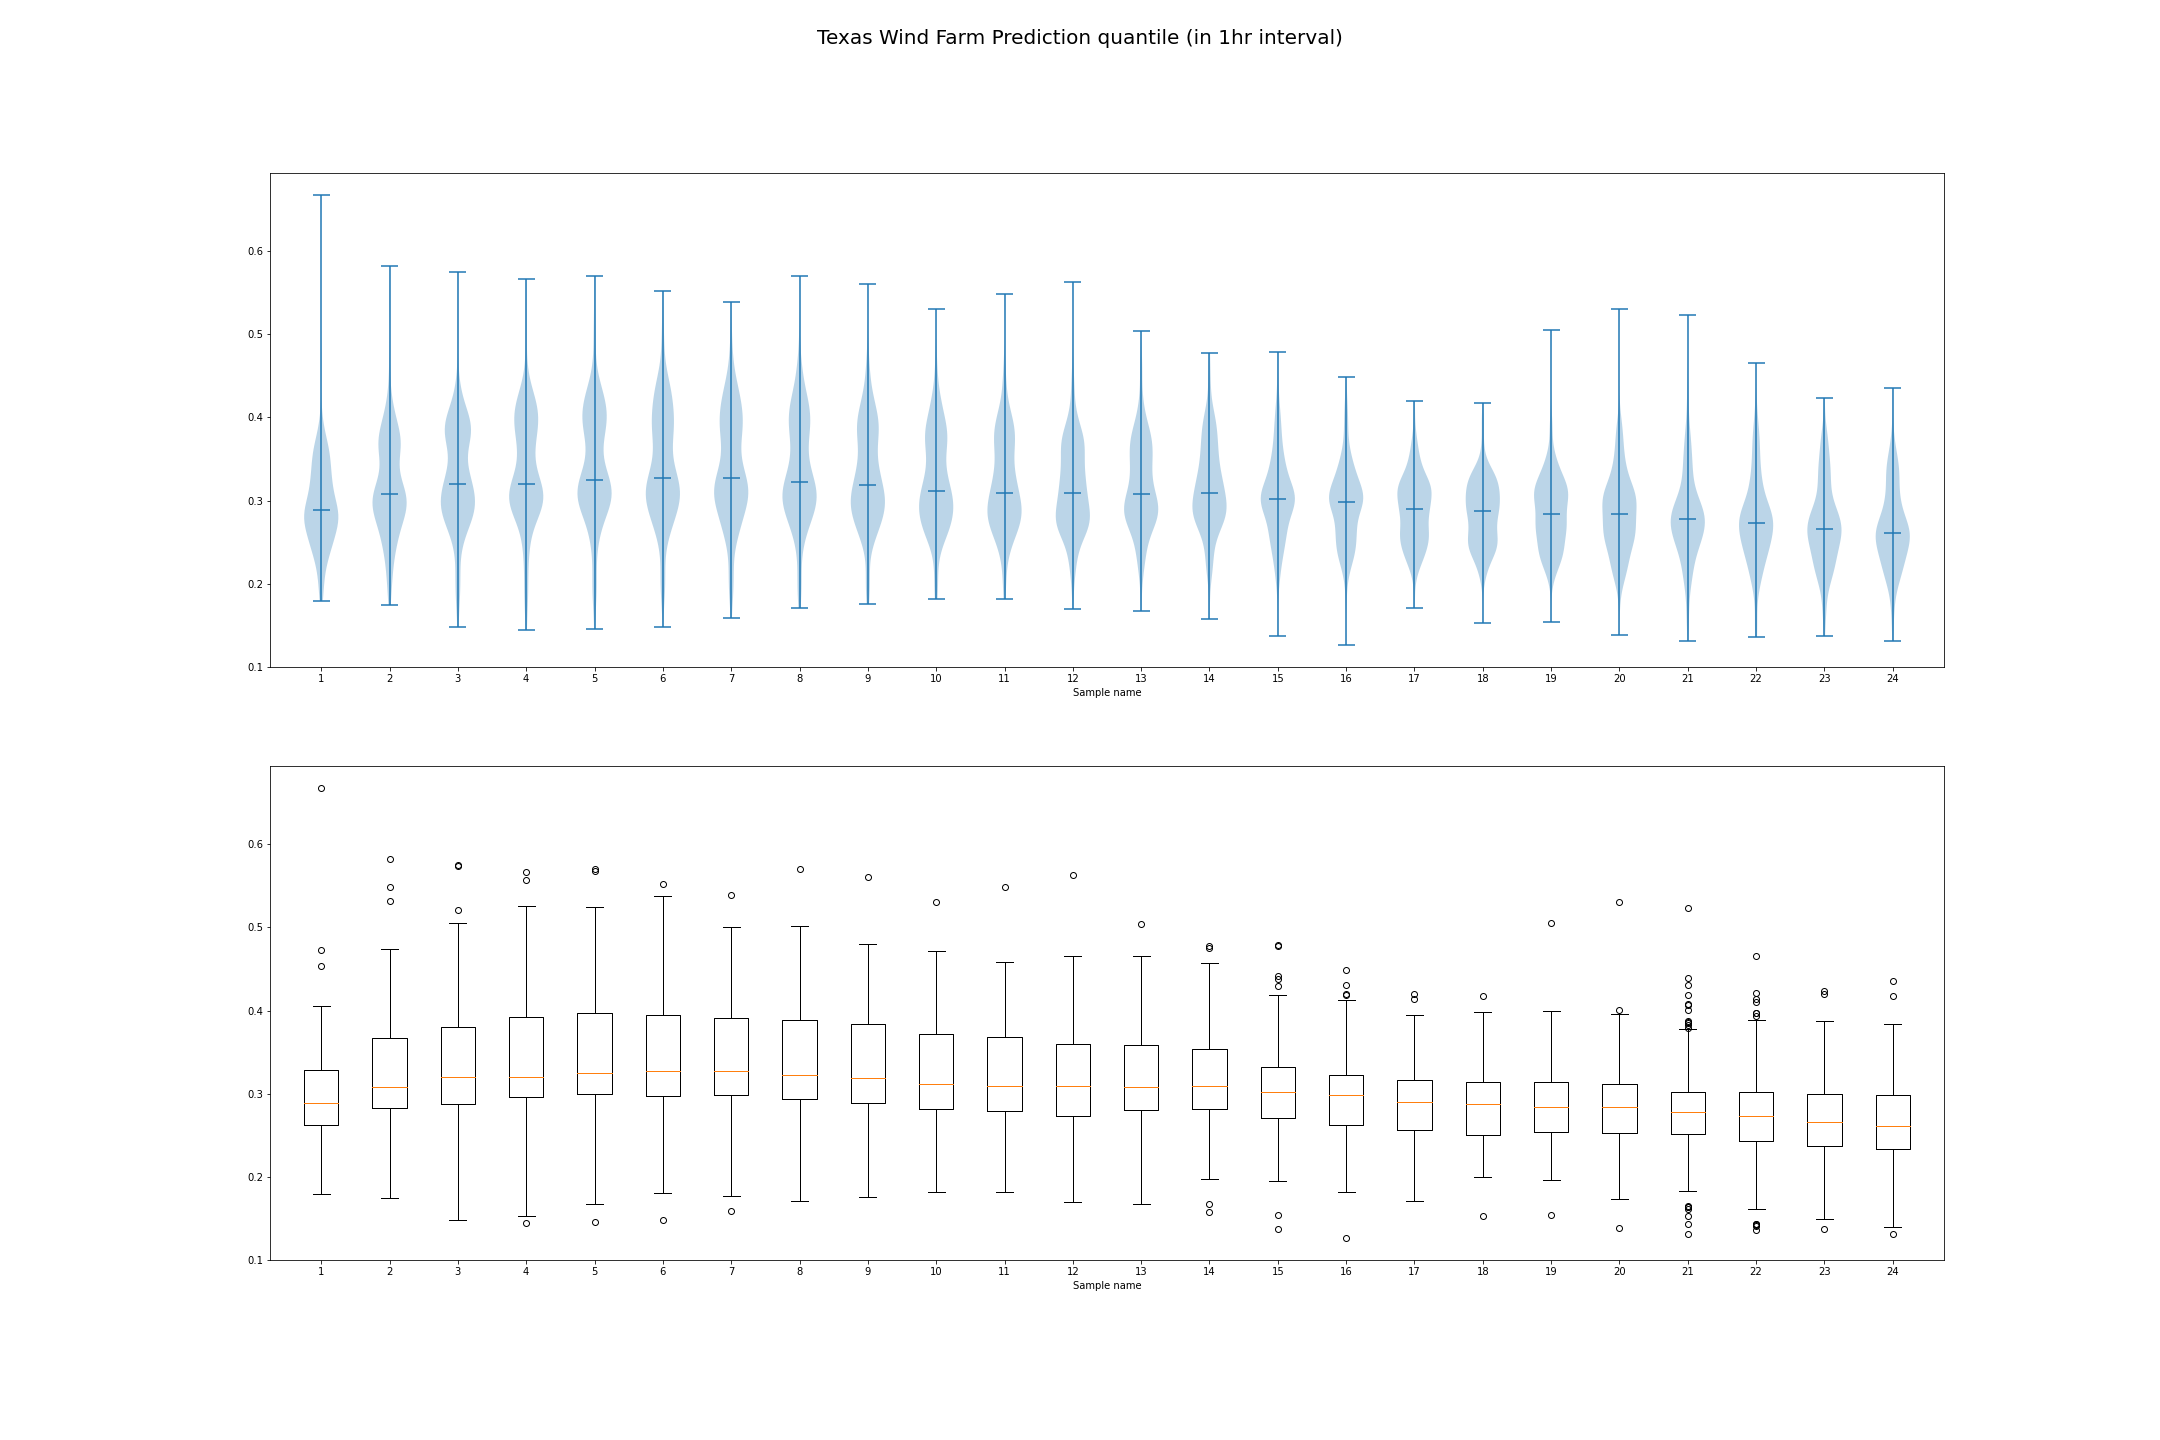
\includegraphics{/Users/teo/Desktop/wind/plots/violin_and_box_quantile_1hr.png}
\caption{Violin and Box of Quantile at 1 Hour Interval}
\end{figure}

We see that, from the above violin and box plot, except at hour 24, the
distribution of quantiles are similar across most of the day time.
During early morning to noon, most of the outliers occurs at the tail of
distribution. At hour 24, the quantile is lower comparing to other
hours.

\hypertarget{quantile-at-24-hour-interval}{%
\subsubsection{Quantile at 24 Hour
Interval}\label{quantile-at-24-hour-interval}}

We are also interested in how \(\mathbf{q}\) is distribution
geographically across all assets, we know that \(\mathbf{q}\) is vector
of length \(J\). Plotting \(\mathbf{q}\) on the map of Texas, we get the
following

\begin{figure}
\centering
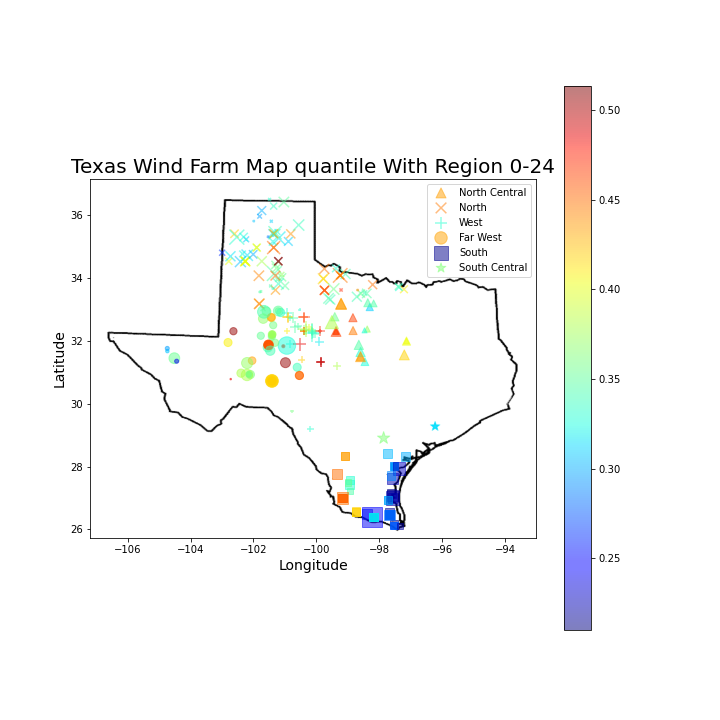
\includegraphics{/Users/teo/Desktop/wind/plots/quantile_24hr_with_area.png}
\caption{Quantile of Bias at Hourly
Interval}
\end{figure}

As shown on the above quantile plot, we see that there is no apparent
spatial relationship across assets on quantile. Some assets at the
Southwest boarder of texas tend to have lower quantile.

\hypertarget{kendalls-coefficient-for-each-region}{%
\subsection{kendall's Coefficient for Each
Region}\label{kendalls-coefficient-for-each-region}}

We are also interested in the ordinal correlation of \(\sigma\) between
each asset across hours. Since there are a total of 6 regions texas and
\(S\) is the entire set of assets. Let

\[S = \{ S_1, S_2, S_3, S_4, S_5,S_6\}\]

Where \(S_i, i \in \{1,2,3,4,5,6\}\) is the set of assets in a
particular region. And let

\[\tau_i^{h}=\frac{2}{|S_i|(|S_i|-1)} \sum_{m<n, m,n \in S_i} \operatorname{sgn}\left(\sigma_{m}^{h}-\sigma_{n}^{h}\right) \operatorname{sgn}\left(\sigma_{m}^{h+1}-\sigma_{n}^{h+1}\right)\]

So \(\tau_i^{h+1}\) is the kendall correlation coefficient for asset
\(S_i\) during hour interval \([h,h+1]\). Then for \(h \in [1,23]\) and
for\(  i \in \{ 1,2,3,4,5,6\}\) we plot out the kendall correlation for
each region across 23 hour intervals,

We also calculated the overall kendall correlation coefficient
\(\tau^h\) by

\[\tau^{h}=\frac{2}{|S|(|S|-1)} \sum_{m<n, m,n \in S} \operatorname{sgn}\left(\sigma_{m}^{h}-\sigma_{n}^{h}\right) \operatorname{sgn}\left(\sigma_{m}^{h+1}-\sigma_{n}^{h+1}\right)\]

\begin{figure}
\centering
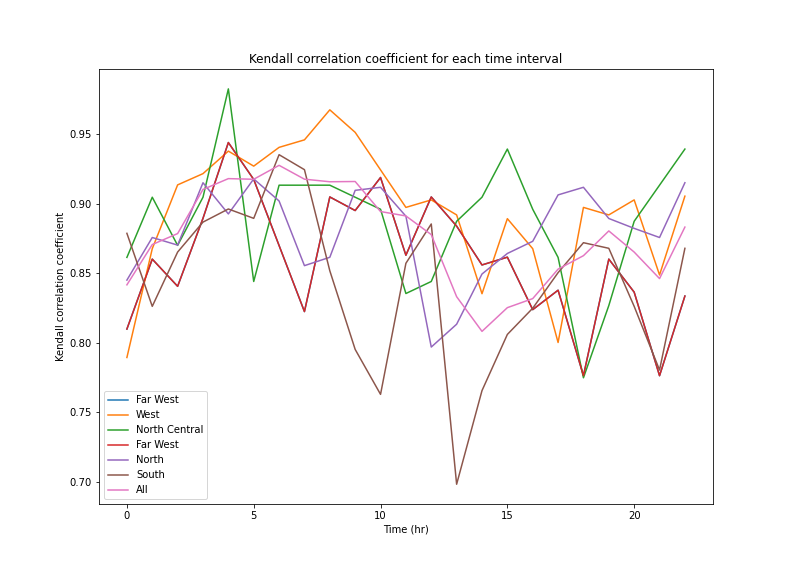
\includegraphics{/Users/teo/Desktop/wind/plots/kendall.png}
\caption{Kendall Coefficient by Area}
\end{figure}

As seen from the plot, overall, the kendall's \(\tau\) tend to be lower
in the afternoon comparing to the mornings. It was also found that the
assets in the South behave unsual comparing to other regions, its
kendall's \(\tau\) is lowest at hour 13.

\hypertarget{capacity-vs--std-of-unnormalized-bias}{%
\subsection{Capacity vs. std of unnormalized
bias}\label{capacity-vs--std-of-unnormalized-bias}}

We are also interested in the correlation between an asset's capacity
and the standard deviation of unormalized bias. Let

\[\tilde{\sigma}= \sqrt{\frac{\sum_{h = 1}^{24}\sum_{d = 1}^{365}\left(\tilde{\beta}_{d,h}-\bar{\tilde{\beta}}\right)^{2}}{365}}\]

Plotting Capacity \(C\) on the x-axis and \(\tilde{\sigma}\) on the y
axis, we calculate the corelation coefficient \(r^2\)

\[r=\frac{\sum_{i = 1}^J\left(\sigma_{i}-\bar{\sigma}\right)\left(C_{i}-\bar{C}\right)}{\sqrt{\sum_{i = 1}^J\left(\sigma_{i}-\bar{\sigma}\right)^{2} \sum\left(C_{i}-\bar{C}\right)^{2}}}\]

where \(\bar{\sigma} = \frac{1}{J} \sum_{i = 0}^J \sigma_i\) and
\(\bar{C} = \frac{1}{J} \sum_{i = 0}^J C_i\)

It was calculated that \(r^2 = 0.897\) indicating a relatively strong
linear relationship. However, from the scatter plot we can see that the
linear relationship is strong for \(C < 450\) . It was also observed
that for \(C>450\) There is a clearly non linear pattern. Besdies, the
assets in the south has lower std/capacity ratio comparing to other
regions. Therefore, we use a local regression to make a better fit of
the data.

With the weight function

\[w(x)=\left(1-|d|^{3}\right)^{3}\]

where \(d\) is the distance of a given data point from the point on the
curve being fitted, scaled to lie in the range from 0 to 1. We also
specify the loss function as

\[\operatorname{RSS}_{x}(A)=\sum_{i=1}^{N}\left(y_{i}-A \hat{x}_{i}\right)^{T} w_{i}(x)\left(y_{i}-A \hat{x}_{i}\right) .\]

Here, \(A\) is an \((n+1) \times(n+1)\) real matrix of coefficients,
\(w_{i}(x):=w\left(x_{i}, x\right)\) and the subscript \(i\) enumerates
input and output vectors from a training set.

\begin{figure}
\centering
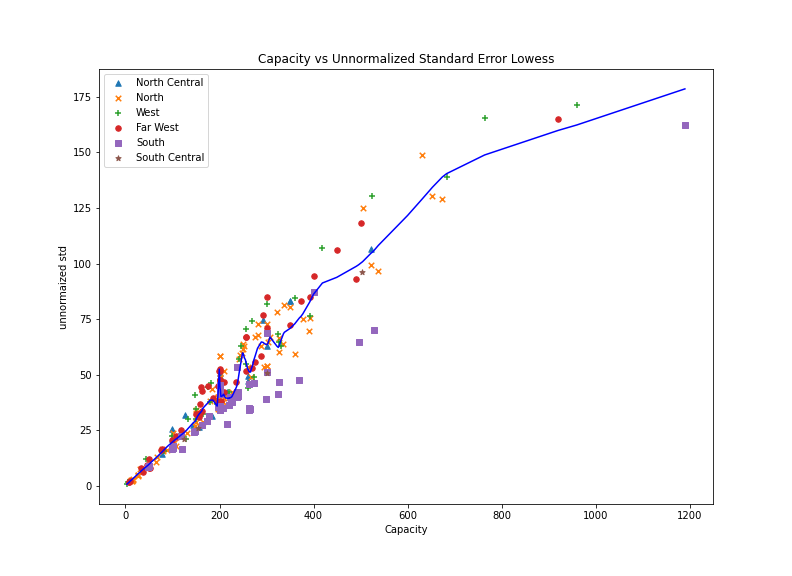
\includegraphics{/Users/teo/Desktop/wind/plots/capacity_vs_unnormstd_lowess.png}
\caption{Capacity vs. Unnormalized std lowess}
\end{figure}

\hypertarget{outliers}{%
\subsection{Outliers}\label{outliers}}

Let outliers to be any oberservation outside the range

\[\left[q^{25}-k\left(q^{75}-q^{25}\right), q^{75}+k\left(q^{75}-q^{25}\right)\right]\]

Where \(q^{25},q^{75}\) are the 25 quantile and 75 quantile
respectively, \(k\) is some non-negative constant. We use \(k=2\) across
all the analysis

\hypertarget{bias-outliers}{%
\subsubsection{Bias Outliers}\label{bias-outliers}}

We count the number of occurence as outliers of each assets across
assets for bias.

\begin{aligned}
&\text { Bias Butliers }\\
&\begin{array}{|l|r|}
\hline \text{Asset} & n_\beta \\
\hline \text { Desert Sky repower } & 19 \\
\hline \text { Canadian Breaks Wind } & 18 \\
\hline \text { Tierra Blanca W } & 16 \\
\hline \text { Broadview Energy JN LLC } & 16 \\
\hline \text { Northdraw Wind } & 16 \\
\hline \text { Wildrose Wind } & 15 \\
\hline \text { Wind Power Partners '94 Wind Farm } & 14 \\
\hline \text { Delaware Mountain Wind Farm } & 14 \\
\hline \text { Gusty Hill Wind } & 14 \\
\hline \text { Pantex Plant Wind Project } & 13 \\
\hline
\end{array}
\end{aligned}

\hypertarget{standard-deviation-outliers}{%
\subsubsection{Standard Deviation
Outliers}\label{standard-deviation-outliers}}

We count the number of occurence as outliers of each assets across
assets for standard deviation of bias.

\begin{aligned}
&\text { Standard Deviation Outliers }\\
&\begin{array}{|l|r|}
\hline \text{Asset} & n_\sigma \\
\hline \text { Cameron } & 10 \\
\hline \text { Anacacho Wind Farm } & 10 \\
\hline \text { San Roman } & 8 \\
\hline \text { Bruenning's Breeze } & 8 \\
\hline \text { Magic Valley } & 8 \\
\hline \text { Gulf Wind Farm } & 7 \\
\hline \text { Penascal II } & 7 \\
\hline \text { Baffin } & 6 \\
\hline \text { Tecovas } 1 \text { W } & 5 \\
\hline \text { Papalote Creek } & 5 \\
\hline
\end{array}
\end{aligned}

\hypertarget{quantile-outliers}{%
\subsubsection{Quantile Outliers}\label{quantile-outliers}}

We count the number of occurence as outliers of each assets across
assets for quantile.

\begin{aligned}
&\text { Quantile Outliers }\\
&\begin{array}{|l|r|}
\hline \text{ Asset} & n_\mathbf{q} \\
\hline \text { Gusty Hill Wind } & 17 \\
\hline \text { Anacacho Wind Farm } & 14 \\
\hline \text { Wind Power Partners '94 Wind Farm } & 14 \\
\hline \text { Delaware Mountain Wind Farm } & 13 \\
\hline \text { Desert Sky repower } & 13 \\
\hline \text { Loma Pinta II } & 12 \\
\hline \text { Loma Pinta Wind } & 12 \\
\hline \text { West Texas Windplant } & 11 \\
\hline \text { Canadian Breaks Wind } & 8 \\
\hline
\end{array}
\end{aligned}

For the above tables, we see that \textbf{Desert Sky repower} has large
bias and quantile, but not standard deviation. The assets on the bias
and quantile tend to align, but large quantile or bias does not mean
they have large standard deviation.

\hypertarget{Standard Deviation vs. Quantile}{%
\subsection{Standard Deviation vs. Quantile}\label{Standard Deviation vs. Quantile}}

For each assets, we made a scatter plot of its standard deviation and quantile

\begin{figure}
  \centering
  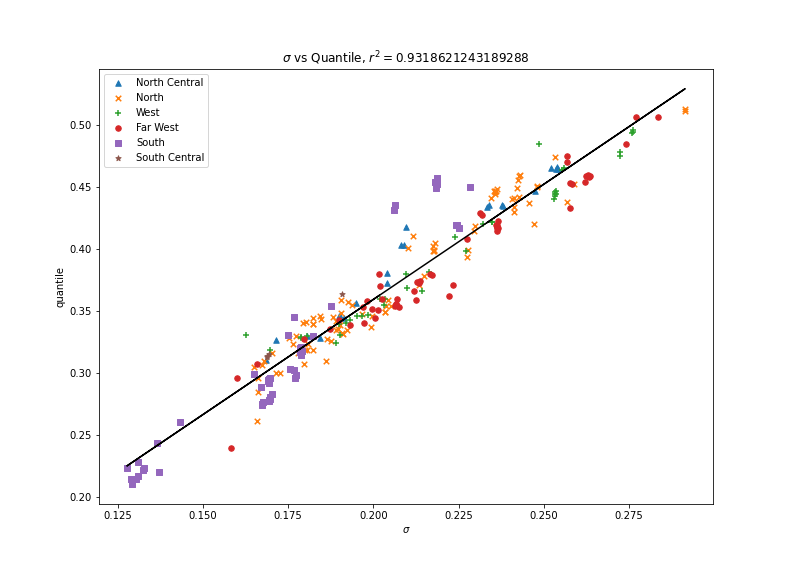
\includegraphics{/Users/teo/Desktop/wind/plots/sigma_vs_quantile.png}
  \caption{Standard Deviation vs. Quantile}
  \end{figure}

\end{document}
